\section{Protokolle}

Protokolle sind �bereink�nfte zweier oder mehrerer Parteien, wie sie miteinander kommunizieren.
Ein menschliches ''Protokoll'' beispielsweise ist eine Sprache. Sie �bermittelt mit Hilfe von
Satzbau und Wortbedeutungen bestimmte Inhalte. Gleiches gilt f�r Protokolle auf Computern oder
innerhalb von Rechnernetzen.
 
\subsection{DHCP}

DHCP, das ''Dynamic Host Configuration Protocol'' ist ein Protokoll, welches einen kleinen
Teil der Netzwerkverwaltung f�r den Administrator einfacher machen soll.\newline
Gew�hnlich werden die oben genannten IP-Adressen auf jedem Rechner einzeln eingestellt.
Dies kann bei gr��eren Netzwerken m�hsam bis un�bersichtlich sein. DHCP schafft hier Abhilfe.

Auf einem Rechner wird die DHCP-Serversoftware installiert. Dort werden die einzelnen
Rechner im Netzwerk mit ihrer Ethernet-Hardware-Adresse und der vom Administrator festgelegten
IP-Adresse eingetragen. Stellt nun ein Rechner im Netzwerk eine Anfrage nach seiner
IP-Adresse, antwortet der DHCP-Server mit dem entsprechenden Wert.\newline
Ein DHCP-Server ist in der Lage, einiges mehr an Werten an einen Rechner zur�ckzuliefern
als eine IP-Adresse. Jedoch ist der Gro�teil davon f�r Administration in der Praxis
recht unwichtig.
 
\subsection{TFTP - der simple Dateitransfer}

TFTP, das ''Trivial File Transfer Protocol'' ist ebenso ein Serverdienst. Er ist mit FTP 
vergleichbar, jedoch wesentlich simpler. So fordert der Server keine Identifikation mit
Benutzername und Passwort.

Im Terminalserver-Betrieb ist TFTP das Protokoll, das das Terminal benutzt, um seinen
Betriebssystem-Startcode (im Falle von Linux der ''Kernel'') herunterzuladen.
 
\subsection{NFS - Dateien �ber das Netzwerk}
 
Das Network File System - NFS - erlaubt das Verwalten von Dateien auf
mehreren Computern innerhalb eines Netzwerkes so, als ob sie auf der lokalen
Festplatte gespeichert w�ren. Dadurch ist es f�r den Benutzer nicht n�tig zu wissen, wo die
Dateien physikalisch gespeichert sind, um auf sie zuzugreifen.
 
�ber NFS hat er von jedem Rechner im Netz gleicherma�en Zugriff auf sein Dateien. Dabei werden die
Dateien vom Server exportiert und vom Terminal importiert:\\
Jedes Terminal kann nur importieren, was der Server ausdr�cklich exportiert!
 
\subsection{X11 - Fenster in der Ferne}   

\begin{figure}

\begin{center}
\resizebox*{!}{7cm}{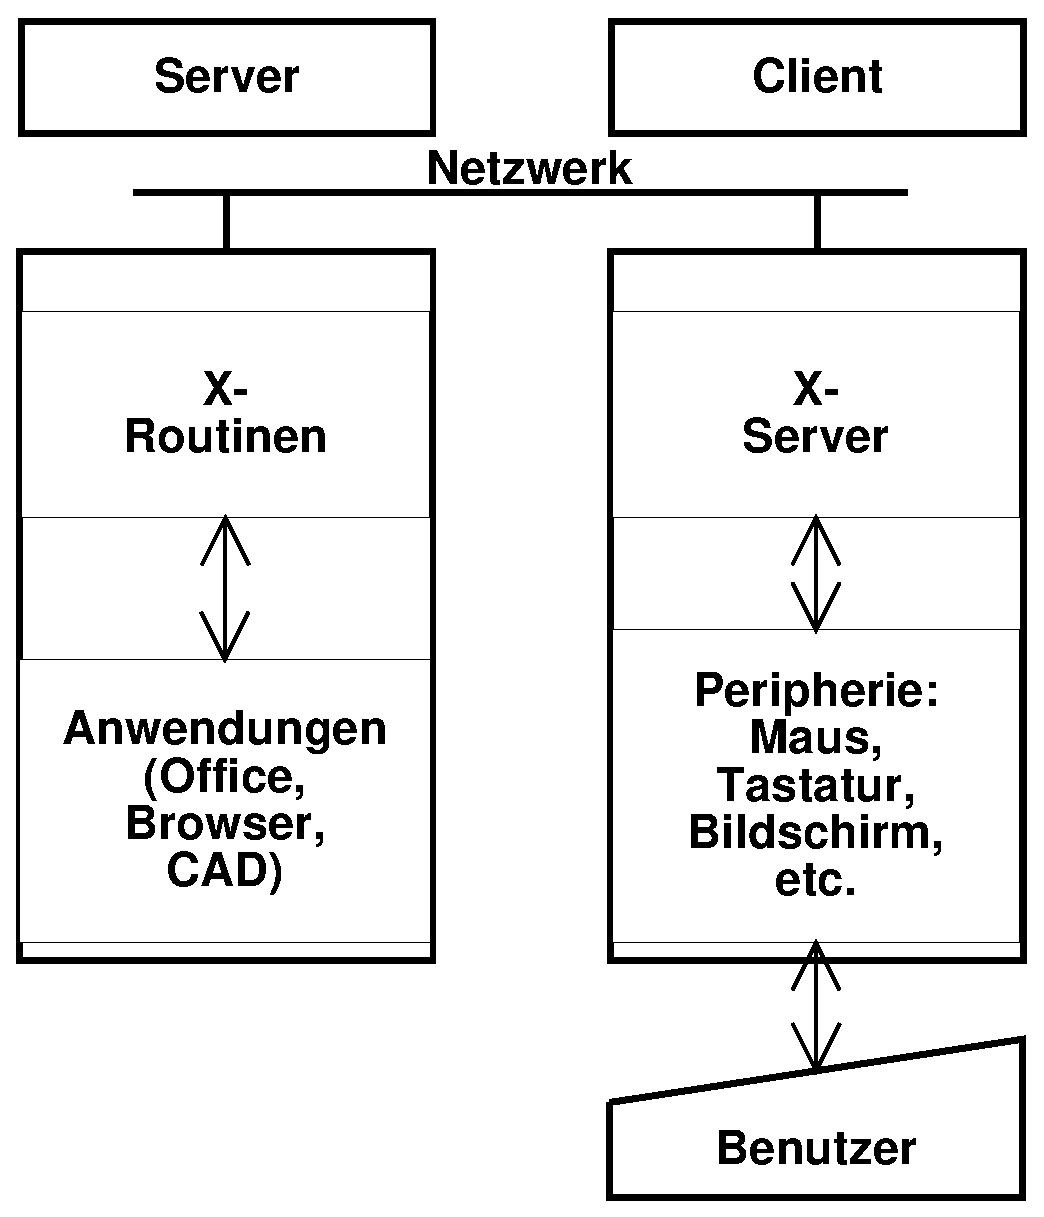
\includegraphics{userguide-networkbasics-protocols-x-flow.eps}}
\end{center}

\caption{Funktionsweise des X11-Protokolls
\label{userguide-networkbasics-protocols-x-flow}}

\end{figure}

X11 ist ein System, welches unter GNU/Linux- und Unix-Systemen die Grafikausgabe regelt.
Das Besondere an ihm ist seine Netzwerkf�higkeit. So kann ein Programm auf einem bestimmten Rechner
laufen, die Anzeige und Bedienung des Programms findet aber auf einem anderen Rechner statt! Im
GNU/Linux- bzw. Unix-Mehrbenutzerbetrieb k�nnen also beliebig viele Rechner
Programme auf einem einzigen Server starten und bei sich anzeigen lassen. Die Zeichnung
\ref{userguide-networkbasics-protocols-x-flow} gibt einen schematischen �berblick.
